\documentclass[parskip=full]{scrartcl}
\usepackage[top=2.5cm, bottom=2.5cm, left=2.5cm, right=2.5cm]{geometry}
\usepackage[utf8]{inputenc}
\usepackage[T1]{fontenc}
\usepackage[german]{babel}
\usepackage{hyperref}
\usepackage[toc, nonumberlist]{glossaries}
\usepackage{graphicx}
\usepackage{enumitem}
\usepackage{float}
\usepackage{color}

\hypersetup{
  colorlinks=false,
  linktoc=all,
  hidelinks,
}

\title{OSIP - Softwaredesign}
\subtitle{OPC UA Simulator for Industrial Plants}
\author{
    M. Armbruster\\
    D. Kahles\\
    H. Lehmann\\
    M. Schwarzmann\\
    N. Wilhelm
}

\begin{document}
\maketitle

\vspace{20px}
\begin{center}
  
\includegraphics[scale=0.4]{../icon.png}
\end{center}
\pagebreak
\tableofcontents
\pagebreak

\section{Einleitung}
Nachdem die Anforderungen an OSIP im Pflichtenheft ausführlich spezifiziert wurden, wird in diesem Dokument
der softwaretechnische Entwurf von OSIP, insbesondere die Klasseneinteilung, erläutert. Makroskopisch wurde OSIP
mit einer \emph{Model View Controller}-Architektur entworfen. Diese ermöglicht beispielsweise
lose Kopplung zwischen Simulation und Anzeige der simulierten Anlage.

Um die Anwendung und Interaktion der entworfenen Klassen zu illustrieren, sind Ausschnitte aus dem Programmablauf
in Form von Sequenzdiagrammen erläutert. Die meisten der Sequenzdiagramme zeigen eine Interaktion über die Grenzen
des jeweiligen Paketes hinweg.

In diesem Dokument ist auch beschrieben, welche der im Pflichtenheft genannten Kann-Kriterien nun tatsächlich
umgesetzt werden und in welchem Umfang die Umsetzung stattfindet. Im Entwurf verwendete Entwurfsmuster werden
ebenfalls in diesem Dokument beschrieben.

\section{Klassenbeschreibungen}
Die Klassenbeschreibungen können im Anhang dieses Dokuments gefunden werden.

\section{Abläufe}
Um die Anwendung und Interaktion der entworfenen Klassen zu illustrieren, sind im Folgenden Ausschnitte aus dem Programmablauf
in Form von Sequenzdiagrammen erläutert. Die meisten der Sequenzdiagramme zeigen eine Interaktion über die Grenzen
des jeweiligen Paketes hinweg. Es werden zentrale und komplexe Abläufe innerhalb von OSIP gezeigt und textuell beschrieben.

Die Sequenzdiagramme sind insbesondere deshalb wichtig, weil dadurch genau die verwendeten Schnittstellen nachgedacht wird
und somit Unklarheiten zwischen den verschiedenen Softwarearchitekten beseitigt werden können.

\subsection{Wrapper für OPC UA}
OSIP verwendet Wrapper für Milo, da Milo eine zu komplexe Schnittstelle bereitstellt.
Viele der angebotenen Funktionen (wie beispielsweise mehrere Namespaces) werden von uns nicht benötigt
und werden durch die Wrapper verborgen. Für die Server-Seite und die Client-Seite wurde je eine Schnittstelle entworfen.
Beide Seiten sollen nun kurz vorgestellt werden. Die komplexen Aufrufe an die Schnittstelle von Milo werden in den
Sequenzdiagrammen gut sichtbar.

\subsubsection{Server-Wrapper}
\begin{figure}[H]
  \centering
  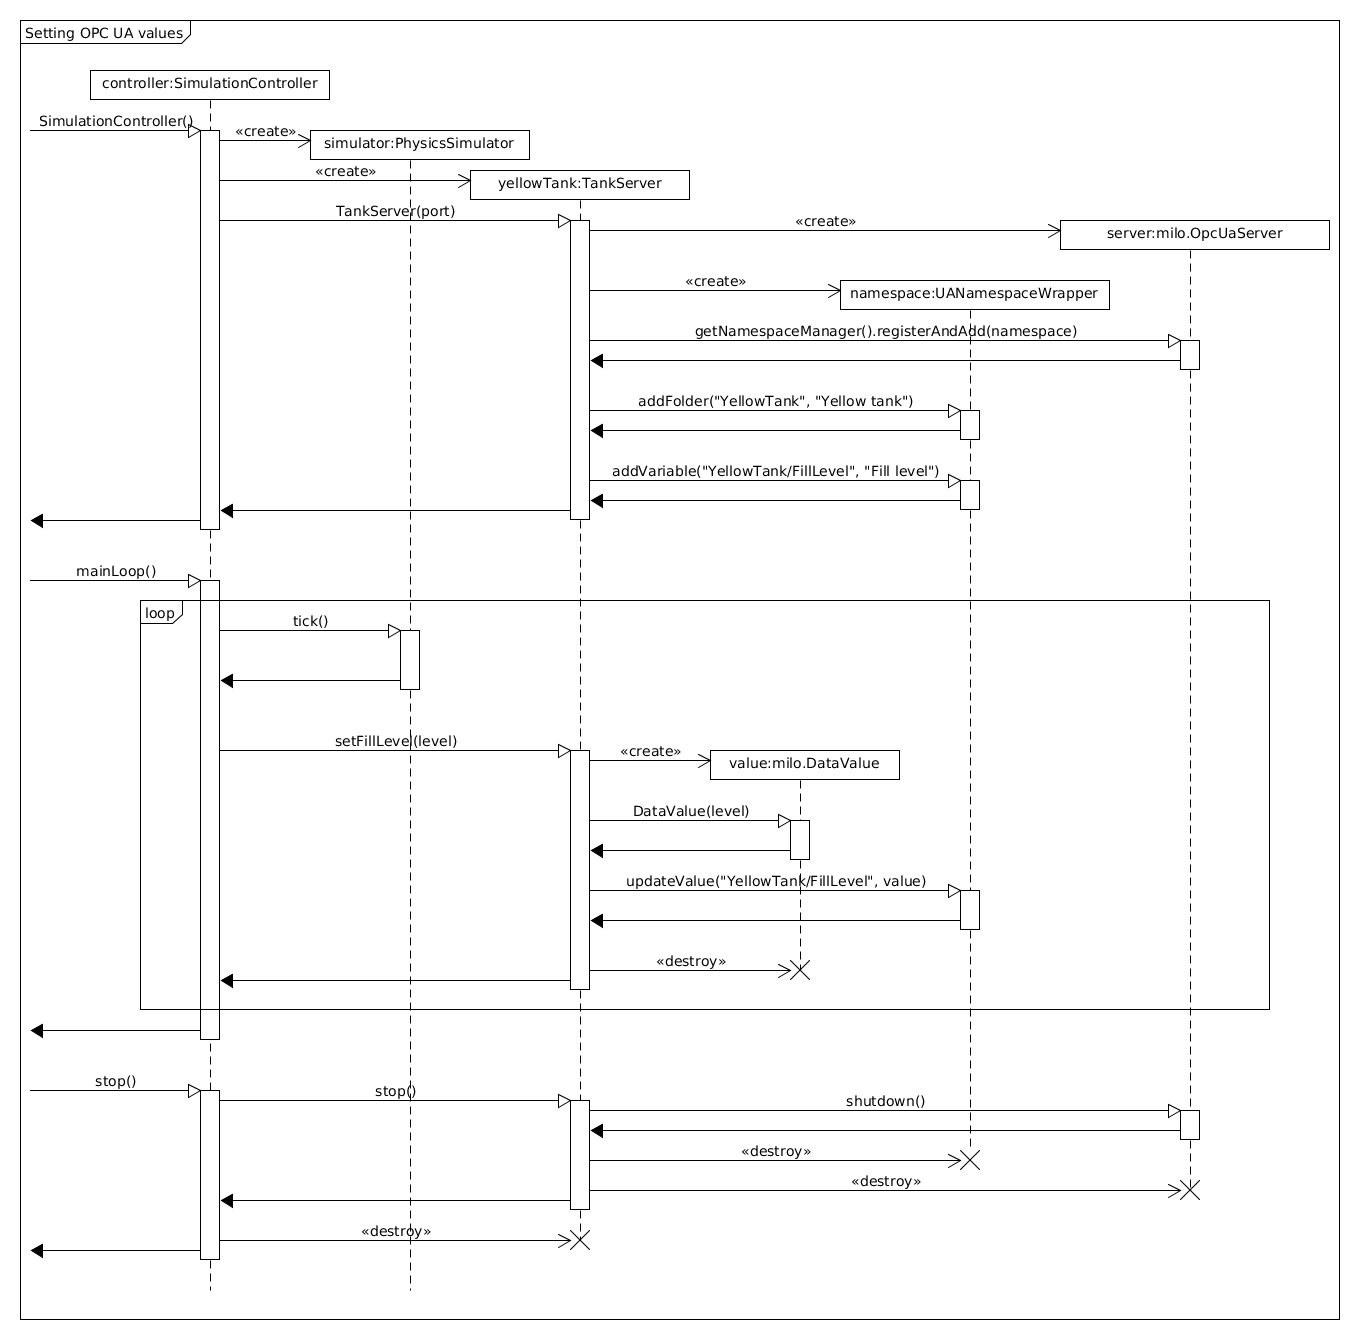
\includegraphics[scale=0.38]{design/sequence-diagrams/sequence-set-server-value.png}
  \caption{Setzen von Werten über den UAServerWrapper}
\end{figure}
Beim Erstellen des Controllers werden auch der Simulator und die Server der Tanks erstellt.
Dieser Server erbt von \emph{UAServerWrapper}, welcher Milo abstrahiert. Wie im Diagramm zu sehen,
werden vom Wrapper Server und Namespace erstellt. Der Namespace wird beim Server registriert und
im Namespace werden die Ordner und Variablen erstellt (hier exemplarisch der Füllstand).

Beim Setzen des Füllstandes wird nur \emph{setFillLevel()} aufgerufen. Der \emph{UAServerWrapper} erstellt daraufhin
ein entsprechendes \emph{DataValue}, das von Milo gebraucht wird, und übergibt es an den Standard-Namespace.
Durch einen Aufruf von \emph{stop()} fährt der \emph{UAServerWrapper} den Server herunter und dereferenziert
Server und Namspace.

\subsubsection{Client-Wrapper}
\label{milo-wrapper-diagram}
\begin{figure}[H]
  \centering
  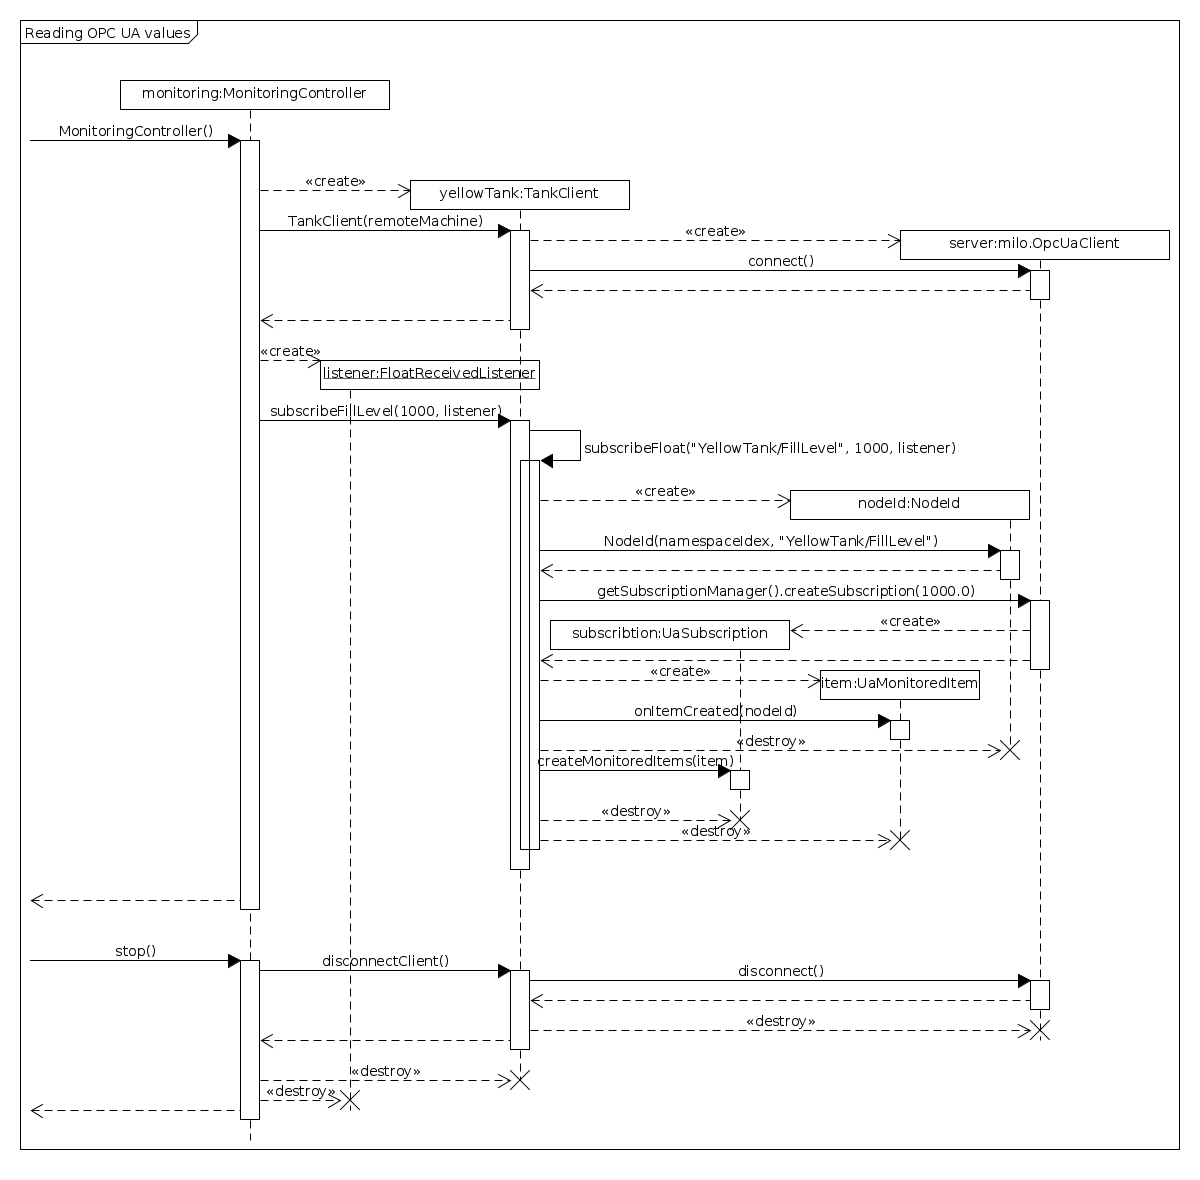
\includegraphics[scale=0.4]{design/sequence-diagrams/sequence-subscribe-client-value.png}
  \caption{Abonnieren von Werten über den UAClientWrapper}
\end{figure}
Der Controller ruft beim \emph{TankServer}, welcher von \emph{UAClientWrapper} erbt, die subscribe-Methode für den entsprechenden Parameter auf
(hier exemplarisch \emph{subscribeFillLevel()}). Der \emph{UAClientWrapper} erstellt ein \emph{NodeId}-Objekt und damit die
entsprechende \emph{ReadValueId}. Diese registriert er beim \emph{OpcUaClient}.
Beim Empfang von Werten wird der entsprechende Listener aufgerufen. Der \emph{UAClientWrapper} übernimmt somit die
komplette Interaktion mit Milo. Die obige Zeichnung ist nicht vollständig. Zum Erstellen einer Subscription bei Milo werden über 10
Objekte erzeugt und gleich wieder dereferenziert, was diesen Rahmen sprengen würden. Die Zeichnung gibt nur einen groben Überblick.

\subsection{Neuzeichnen der GUI der Simulation}
  Das Aktualisieren der GUI der Fertigungssimulation erfolgt in regelm\"a{\ss}igen Abst\"anden. Das Hauptfenster tr\"agt dazu seinen Komponenten auf,
  sich selbst an passender Stelle im Fenster neu zu zeichnen. Hier ist der Vorgang nur beispielhaft an den Tanks gezeigt. Er funktioniert
  f\"ur die anderen Komponenten analog.
  \begin{figure}[H]
    \centering
    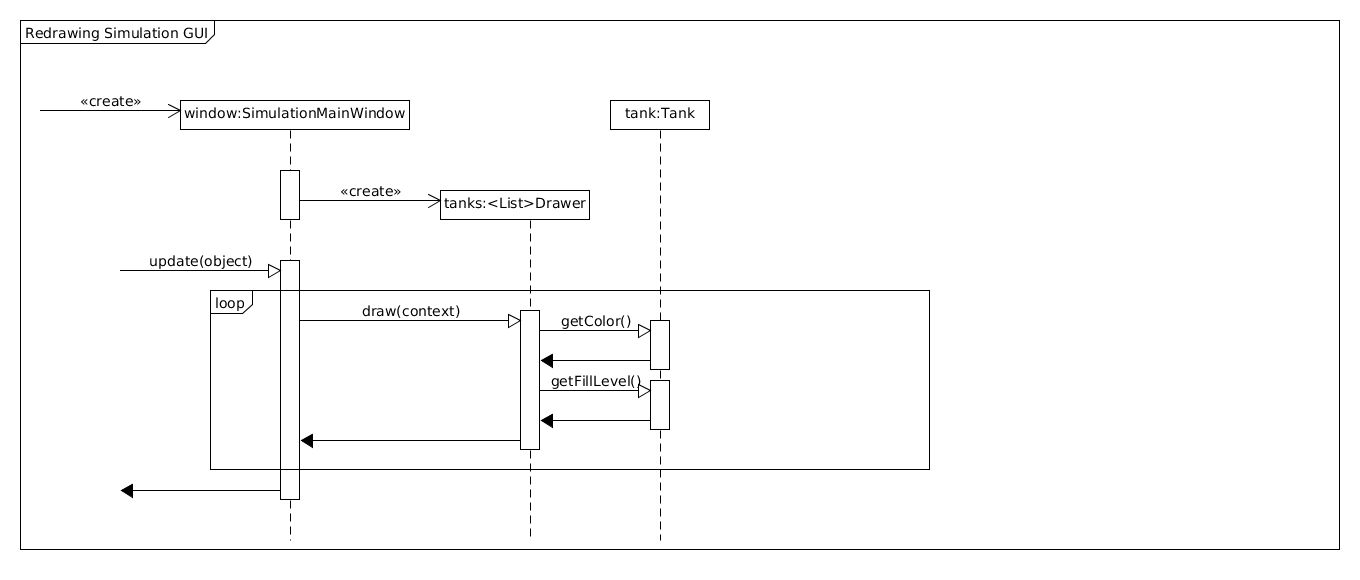
\includegraphics[scale=0.35]{design/sequence-diagrams/simulation-redraw.png}
    \caption{Neuzeichnen der GUI der Simulation}
  \end{figure}
  Bei der Erzeugung des Hauptfensters instanziiert dieses einen neuen \emph{GraphicsContext}, der die Schnittstelle zum Canvas darstellt.
  Anschlie{\ss}end werden die einzelnen Grafikkomponenten, die \emph{Drawer}, erstellt und mit Ihrer jeweiligen Position versehen.
  Daraufhin wird der \emph{UpdateThread} erzeugt und dessen \emph{start()} Methode aufgerufen. Diese l\"o{\ss}t periodisch das
  Neuzeichnen der GUI aus.\\
  Das Neuzeichnen wird \"uber die Methode \emph{draw()} der einzelnen Komponenten ausgel\"o{\ss}t. Dabei veranlasst der \emph{UpdateThread}, dass sich jeder \emph{Drawer}
  selbst neu zeichnet. Als anonyme Klasse besitzt der \emph{UpdateThread} die M\"oglichkeit, die \emph{Drawer} anzusprechen. Im Falle der 
  \emph{TankDrawer} fragen diese erst die aktuellen Werte vom jeweils zugeordneten \emph{Tank} der Fertigungssimulation ab, um anschlie{\ss}end
  \"uber Aufrufe an den \emph{Context} die neue Darstellung zu veranlassen.

\subsection{Berechnung der Tank-Simulation}
\begin{figure}[H]
  \centering
  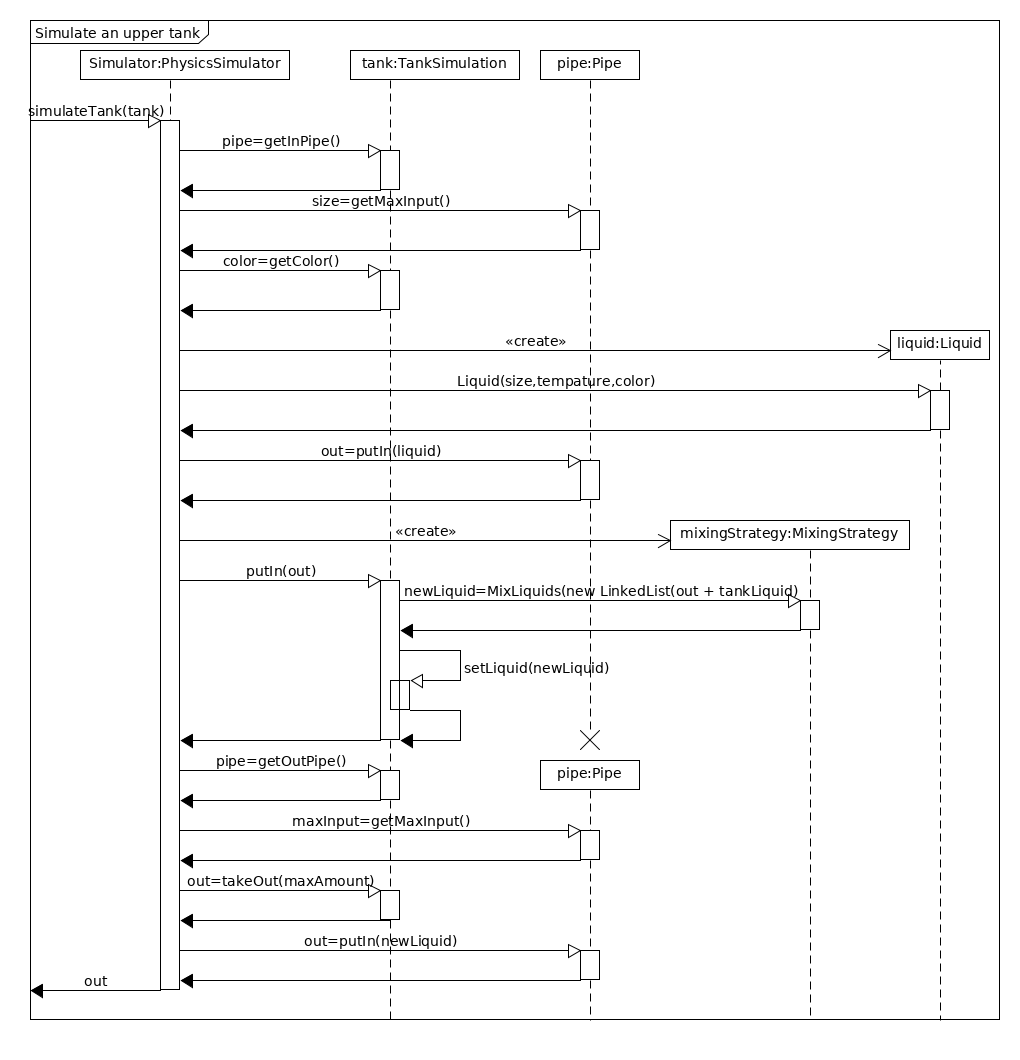
\includegraphics[scale=0.45]{design/sequence-diagrams/tank-simulation.png}
  \caption{Berechnung der Tank-Simulation}
\end{figure}
Dies ist die Simulation eines der oberen Tanks. Für die vollständige Simulation muss \emph{simulateTank()} für jeden Tank aufgerufen
und die Rückgabewerte zum Mixtank hinzugefügt werden. Zuerst erfragt die Simulation beim Tank die Leitung, die zum Tank hinführt, und ermittelt
mit \emph{getMaxInput()} die maximale Durchflussmenge. Anschließend muss berechnet werden, welche Farbe die Flüssigkeit haben soll, die in den Tank
hinein fließt. Dazu wird der TankSelector Enum-Wert vom Tank geholt, und damit die Funktion \emph{getInitialColor()} aufgerufen, die die initiale Farbe der Tanks definiert.
Dann kann ein neues \emph{Liquid} Objekt erstellt werden, das so groß ist, dass es gerade noch in die Leitung passt. Mittels \emph{putIn()} wird es
in die Leitung gesteckt. Der Rückgabewert von \emph{putIn()} ist die Flüssigkeit, die am anderen Ende der Leitung herauskommt. Diese wird dann in den
Tank eingefügt. Dazu verwendet der Tank eine \emph{SubtractiveMixingStrategy}, um die Farben und Temperaturen zu mischen. Nachdem die Flüssigkeiten
gemischt sind, wird die Leitung vom oberen Tank zum Mixtank geholt und ermittelt, wie viel Flüssigkeit dort hineinpasst. Diese Menge wird dann aus dem
Tank herausgenommen und in diese Leitung hineingesteckt. Der Rückgabewert von \emph{simulateTank()} ist dann die Flüssigkeit, die am Ende der Leitung
(also beim Mixtank) herauskommt. Diese Flüssigkeit kann die Simulation dann in den Mixtank einfügen (nicht mehr in diesem Diagramm dargestellt).

\subsection{Einstellungen aus der Datei erhalten und verwenden}
\begin{figure}[H]
  \centering
  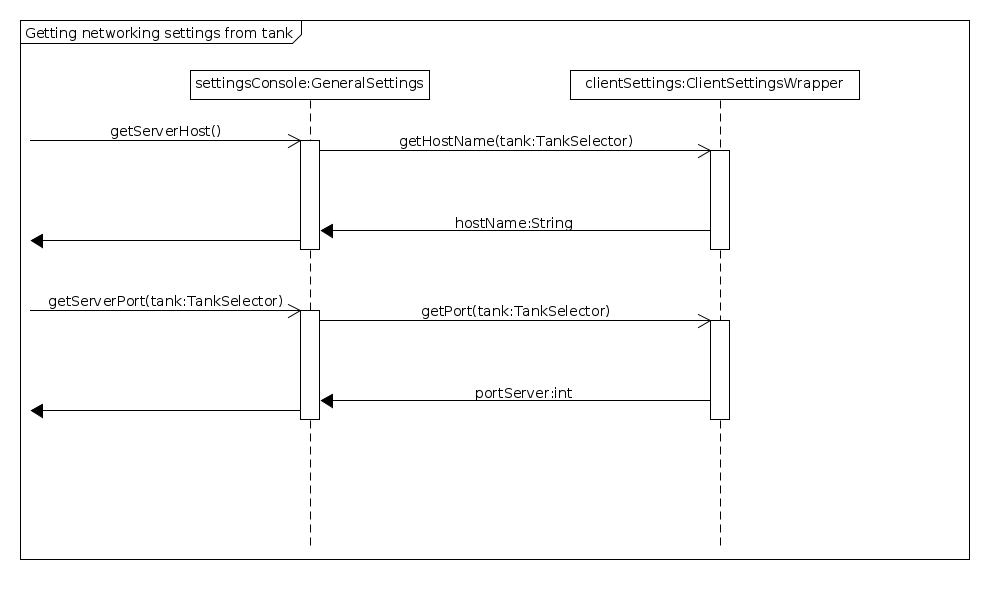
\includegraphics[scale=0.4]{design/sequence-diagrams/getting-networking-settings.png}
  \caption{Einstellungen aus der Datei erhalten und verwenden}
\end{figure}
Bei der Erstellung eines \emph{TankClient} werden Hostname und Port des zugehörigen Servers vom \emph{MonitoringController} mit \emph{getHostName()}
und \emph{getPort()} vom \emph{ClientSettingsWrapper} abgerufen. Eine Instanz des \emph{ClientSettingsWrapper}s
ist im \emph{MonitoringController} zu finden. Es wird eine \emph{RemoteMachine} erstellt und mit Hostname und Port konfiguriert.
Danach erstellt man einen \emph{TankClient}, der die \emph{RemoteMachine} übergeben bekommt und sich mit dem Server verbinden kann.

\subsection{Start der Überwachungskonsole}
\begin{figure}[H]
	\centering
	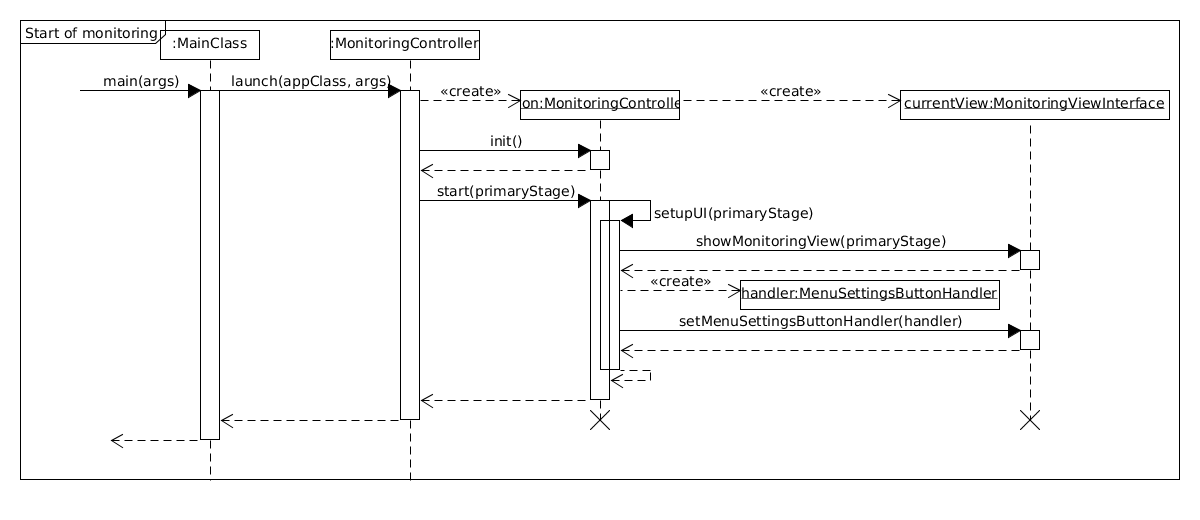
\includegraphics[scale=0.4]{design/sequence-diagrams/start-of-monitoring.png}
	\caption{Start der Überwachungskonsole}
\end{figure}
Beim Start der Überwachungskonsole wird über die \emph{main()} Methode die statische \emph{launch()} Methode der Oberklasse \emph{javafx.application.Application} von \emph{MonitoringController} aufgerufen. Diese ist für den eigentlichen Startvorgang verantwortlich und initialisiert unter anderem JavaFX.
Im Laufe des Startvorgangs wird eine Instanz des \emph{MonitoringControllers} erstellt, die die Verbindung zwischen der Ansicht der Überwachungskonsole und dem Modell herstellt. Dazu erstellt es beispielsweise die Ansicht innerhalb der Methode \emph{setupUI()} über das \emph{MonitoringViewInterface} sowie alle Handler, wobei der \emph{MenuSettingsButtonHandler} als ein Beispiel dargestellt ist.

\subsection{Speichern der Einstellungen}
\begin{figure}[H]
	\centering
	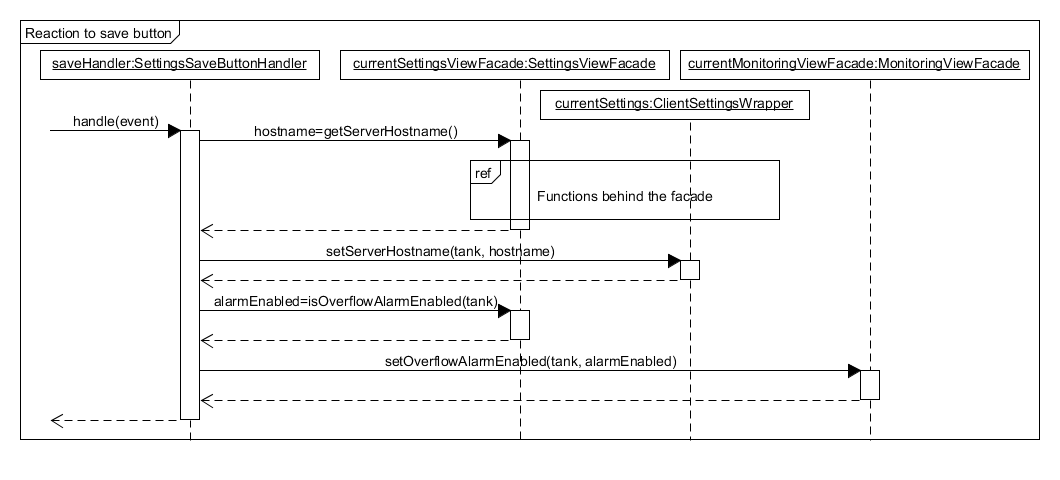
\includegraphics[scale=0.4]{design/sequence-diagrams/save-settings.png}
	\caption{Speichern der Einstellungen}
\end{figure}
Wird in den Einstellungen der Überwachungskonsole der "`Speichern"'-Knopf gedrückt, löst dieses Ereignis die Methode \emph{handle()} in einer Instanz des \emph{SettingsSaveButtonHandlers} aus.
Dort werden alle vom Benutzer getätigten Einstellungen über die \emph{SettingsViewFacade} ausgelesen und in den \emph{ClientSettingsWrapper} zum Speichern geschrieben, sowie bestimmte Änderungen über die \emph{MonitoringViewFacade} direkt in der Ansicht dargestellt.
Beispielhaft wird das Auslesen und Setzen des Hostnamens für die OPC UA Server und eines Überlaufalarms gezeigt.

\subsection{Funktionsweise der ViewFacades der Überwachungskonsole}
\begin{figure}[H]
	\centering
	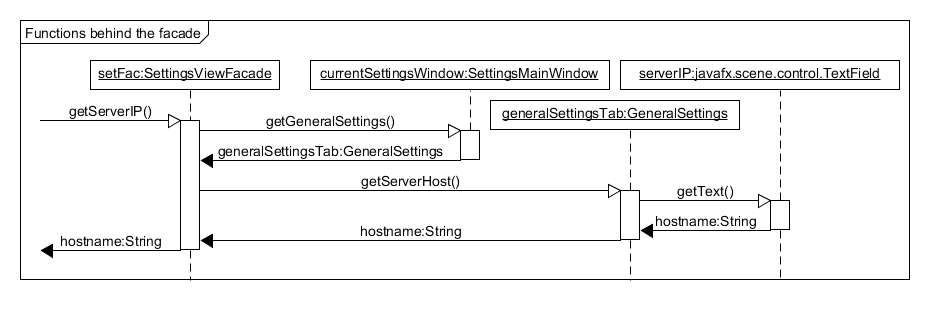
\includegraphics[scale=0.4]{design/sequence-diagrams/functions-behind-the-facade.png}
	\caption{Funktionsweise der ViewFacades der Überwachungskonsole}
\end{figure}
Jeder Aufruf einer Methode der \emph{MonitoringViewFacade()} oder \emph{SettingsViewFacade()} wird an die dahinter liegenden Objekte delegiert, um an den eigentlichen Wert zu kommen oder die eigentliche Operation auszuführen. Das beispielhafte Vorgehen der \emph{SettingsViewFacade} zeigt, wie der Hostname der OPC UA Server vom eigentlichen \emph{javafx.scene.control.TextField}, über den der Benutzer den Hostnamen eingestellt hat, an die \emph{SettingsViewFacade} zurückgereicht wird.

\pagebreak
\section{Änderungen zum Pflichtenheft}

\subsection{\"Ubernommene Kann-Kriterien}
Im Folgenden werden die Kann-Kriterien aus dem Pflichtenheft noch einmal alle aufgelistet. Zu jedem der Kriterien wird
kurz zusammengefasst, was genau es bedeutet. Es werden erst die implementierten und anschlie{\ss}end die nicht implementierten
Kriterien gelistet.

\subsubsection{Implementierte Kann-Kriterien}
Die implementierten Kann-Kriterien sind wie folgt:

\begin{itemize}
    \item Sowohl in der \"Uberwachungskonsole als auch in der Fertigungssimulation werden Fehler bei der Programmausf\"uhrung
    nach stdout geloggt. Die Logs werden nicht persistiert.
    \item In der Fertigungssimulation k\"onnen vorgefertigte Simulationsszenarien geladen werden. Diese sind in eigenen Dateien definiert.
    Die Ausführung der Simulationsszenarien f\"uhrt dazu, dass die Prozessvariablen sich nach Vorgaben des Szenarios ohne
    weitere Aktion des Benutzers \"andern.
    \item In den Zuflusswerten der Fertigungssimulation ist ein Jitter eingebaut. Dieser sorgt f\"ur leichte Variationen in den
    Zuflussmengen und der Temperatur der Zufl\"usse. Das Stärke des Jitters ist nicht einstellbar.
    \item Innerhalb der \"Uberwachungskonsole kann der Benutzer selbst einstellen, in welchem Zeitintervall die Werte der
    Fertigungssimulation abgefragt werden. Alle Werte werden im jeweils gleichen Intervall abgefragt.
    \item Die Alarme in der \"Uberwachungskonsole k\"onnen vom Benutzer jeweils einzeln zu- und abgeschaltet werden. Die Menge der
    aktivierten Alarme wird beim Beenden der \"Uberwachungskonsole persistiert. Beim n\"achsten Start der \"Uberwachungskonsole
    werden die gleichen Alarme automatisch wieder aktiviert.
    \item Die Alarme, die von der \"Uberwachungskonsole empfangen werden, werden in einem Textfenster innerhalb der
    \"Uberwachungskonsole geloggt.
\end{itemize}

\subsubsection{Nicht implementierte Kann-Kriterien}
Die nicht implementierten Kann-Kriterien sind wie folgt:

\begin{itemize}
    \item Es stehen keine verschiedenen Sprachoptionen f\"ur \"Uberwachungskonsole und Fertigungssimulation zur Verf\"ugung.
    Die einzige vorhandene Sprache ist Englisch. Durch die Verwendung von \emph{java.util.ResourceBundle} ist die Anwendung allerdings leicht übersetzbar.
    \item Die vorgegebenen Alarme k\"onnen nicht ver\"andert werden. Insbesondere ist es nicht m\"oglich, eigene Alarme hinzuzuf\"ugen
    oder die Schwellenwerte der vorgegebenen Alarme zu modifizieren.
    \item Der Jitter in den Simulationswerten ist fest vorgegeben und kann in seiner Intensit\"at nicht ver\"andert werden.
    \item Fehler bei der Programmausf\"uhrung werden nicht in eine Datei geschrieben.
\end{itemize}

\section{Klassendiagramme und Paketstruktur}
Das Klassendiagramm kann im Anhang dieses Dokuments gefunden werden. Dabei ist zu beachten, dass die Variable \$SIM\_STEP\_SIZE eine Konstante ist,
die definiert wie granular die Simulation berechnet wird. Davon ist beispielsweise die Klasse \emph{Pipe} abhängig. Der genaue Wert dieser
Konstanten ist noch unbekannt und wird während der Implementierung ermittelt. Zum besseren Verständnis des Diagramms ist im Folgenden
eine grobe Übersicht über die entworfenen Pakete und ihre Anordnung im Klassendiagramm gegeben.

\begin{figure}[H]
  \centering
  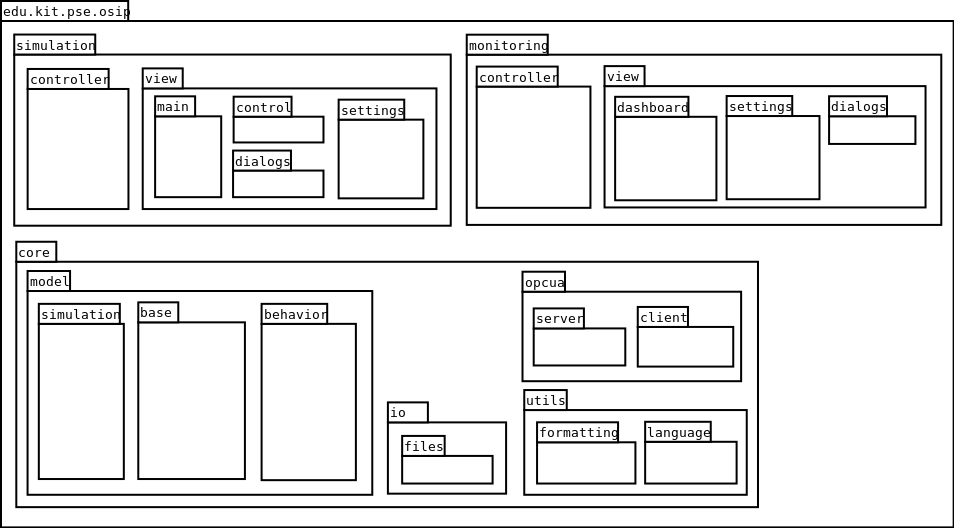
\includegraphics[scale=0.45]{design/class-diagram-map.png}
  \caption{Übersicht über das Klassendiagramm}
\end{figure}

Da die Fertigungssimulation und die Überwachungskonsole eigenständige Programme sind, ist es sinnvoll, diese in getrennten Paketen zu
implementieren. Dazu haben wir die Pakete \emph{simulation} (für die Fertigungssimulation) und \emph{monitoring} (für die Überwachungskonsole)
gewählt. Details zu diesen beiden Paketen gibt es in Kapitel \ref{mvc}. Da viele Funktionalitäten in beiden Programmen
benötigt werden, gibt es außerdem ein Paket \emph{core}, das gemeinsame Funktionalität enthält.

Darin gibt es ein Unterpaket für das Model
der Model-View-Controller Architektur (siehe \ref{mvc}), da für beide Programme das selbe Model verwendet wird. Das Model ist wiederum in
drei Unterpakete unterteilt. Zum einen gibt es das Paket \emph{base}, das den Zustand der Produktionsanlage mit allen Tanks und Leitungen beschreibt.
Eine Simulation ist aber in diesem Paket nicht enthalten, da die Überwachungskonsole dies nicht benötigt. So kann einem Tank beispielsweise keine Flüssigkeit hinzugefügt oder entnommen werden,
sondern nur der komplette Inhalt auf einmal gesetzt werden. Da die Simulation diese Simulationskomponenten jedoch benötigt,
gibt es das Paket \emph{simulation}, dass \emph{base} um solche Simulationskomponenten erweitert. Das dritte Unterpakt des Models ist \emph{behavior}.
Darin sind Klassen enthalten, die nicht den Zustand der Produktionsanlage beschreiben, sondern Aktionen sind, z.B. Alarme und Szenarien.

Außerdem gibt es in \emph{core} ein Unterpaket \emph{io}, dass das Einlesen und Parsen von Konfigurationsdateien für beide Programme enthält. Dann gibt
es ein Unterpaket \emph{opcua}, dass die Verwendung von Milo kapselt und vereinfacht, da das Interface von Milo für OSIP viel zu mächtig
ist (siehe \ref{milo-wrapper-diagram}. Zuletzt gibt es ein Unterpaket \emph{utils}, das weitere gemeinsame Funktionalität wie Internationalisierung oder das Überprüfen von
Formaten beinhaltet.

\pagebreak
\section{Verwendete Entwurfsmuster}
\subsection{Model View Controller f\"ur die Fertigungssimulation}
\label{mvc}
Die Fertigungssimulation ist nach dem Prinzip Model-View-Controller aufgebaut.
Das Model beinhaltet dabei die interne Darstellung der Produktionsanlage sowie die interne Logik, nach der die Produktionsanlage funktioniert
(Pakete \emph{core.model.base}, \emph{core.model.simulation} und \emph{core.model.behaviour}.
Die View erh\"alt die Daten vom Model und stellt diese passend grafisch dar. Sie enth\"alt zudem die M\"oglichkeit f\"ur den Benutzer, Eingaben zu
t\"atigen. Sofern Eingaben erfolgen, werden diese an den Controller weiter gereicht, sodass dieser darauf reagieren kann.
Der Controller steuert das Programm und reagiert auf Benutzereingaben. Dazu veranlasst er einerseits, dass in regelm\"a{\ss}igen Intervallen der
n\"achste Simulationsschritt ausgef\"uhrt wird. Andererseits veranlasst er, je nach Nutzereingabe, dass die Parameter der Simulation ge\"andert werden
und f\"ur die kommenden Simulationsschritte in der ge\"anderten Form verwendet werden. Der Controller steuert zudem die OPC UA Server an, die die
Werte f\"ur die OPC UA Clients der \"Uberwachungskonsole bereitstellen.

\subsection{Model View Controller f\"ur \"Uberwachungskonsole}
Das Programm der \"Uberwachungskonsole ist ebenfalls nach dem Prinzip Model-View-Controller aufgebaut.
Da es die Produktionsanlage nicht simulieren muss, besteht das Model nur aus dem Paket \emph{core.model.base} und \emph{core.model.behaviour}.
Die View benachrichtigt den Controller zu Benutzereingaben, sodass dieser darauf reagieren kann. Die Eingaben dienen hier der Steuerung und Konfiguration
der \"Uberwachungskonsole, z.B. die Einstellung der anzuzeigenden Daten.
Der Controller steuert das Programm und reagiert auf Benutzereingaben. Dazu veranlasst er einerseits, dass in regelm\"a{\ss}igen Intervallen die Daten der
Fertigungssimulation abgefragt werden und steuert die OPC UA Clients an, die der Kommunikation mit der Fertigungssimulation dienen.

\pagebreak
\subsection{Fassaden-Muster: UAServerWrapper, UAClientWrapper}
\begin{figure}[H]
  \centering
  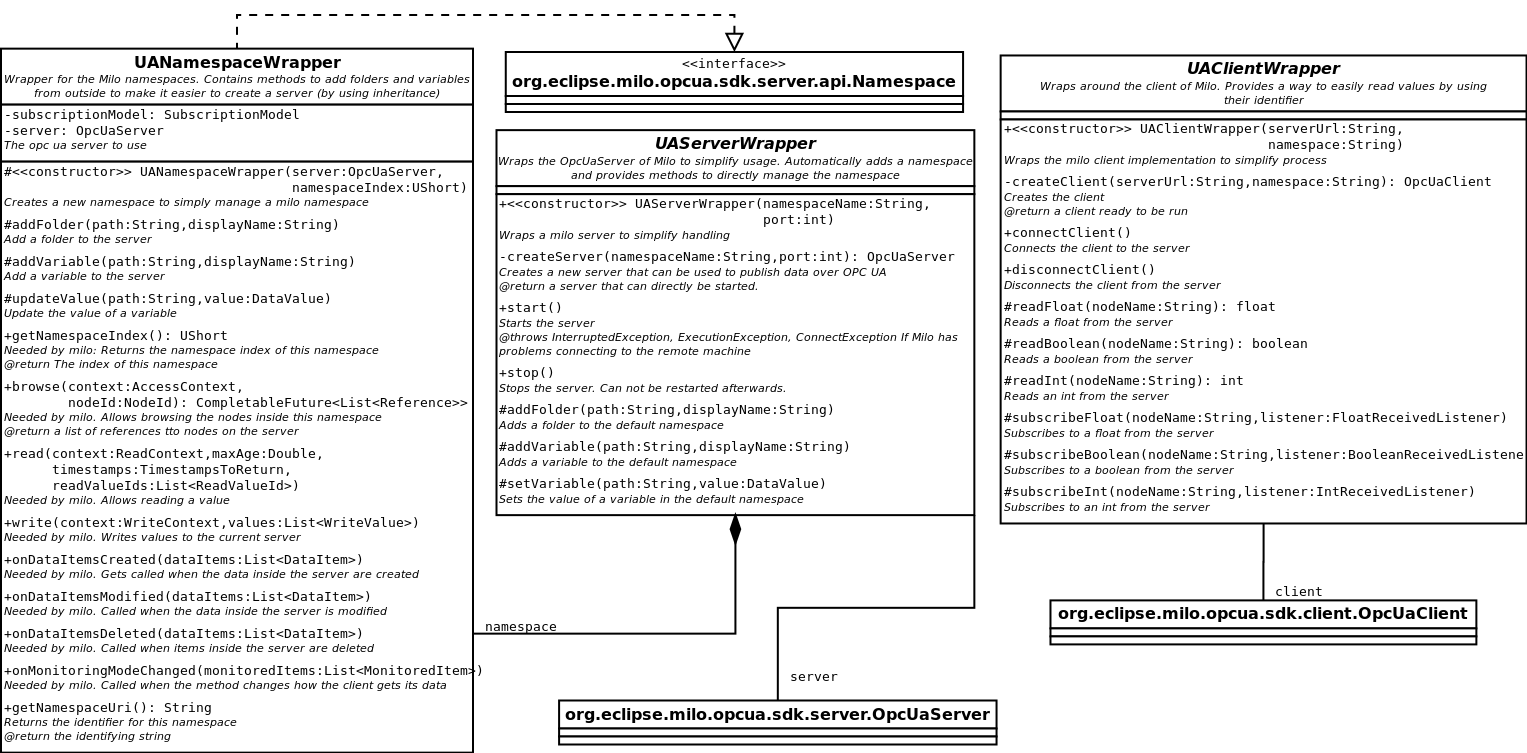
\includegraphics[scale=0.3]{design/pattern-screenshots/fascade-UAWrapper.png}
  \caption{Ausschnitt aus dem Klassendiagramm: Fassade in Milo-Wrappern}
\end{figure}
Milo besitzt eine sehr komplexe Schnittstelle, zu deren Benutzung man sich ausgiebig mit dem oft schlecht dokumentierten Code
der Library beschäftigen muss (Zertifikate manuell deaktivieren etc.). Des Weiteren unterstützt Milo mehr Funktionalität,
als sie in unserem Kontext gebraucht wird (mehrere Namespaces etc.).

Das Fassaden-Muster ist dazu da, um Schnittstellen zu vereinfachen und vereinheitlichen.
Der \emph{UAServerWrapper} erstellt automatisch einen Standard-Namespace und leitet Anfragen an
diesen weiter. Zusätzlich wird das Starten des Servers durch Verstecken von Initialisierungen vereinfacht. Der \emph{UAClientWrapper}
bietet Methoden, um Werte bestimmter Typen direkt und synchron vom Server abzurufen. Die Werte können hierbei direkt über ihren
Namen angesprochen werden - die Umsetzung in \emph{NodeId}s entfällt über die Fassade.

Wir haben das Muster gewählt, um allen
Beteiligten die Handhabung von Milo zu erleichtern. Durch die Fassade muss sich nur noch eine Person damit beschäftigen, wie
Milo intern zu benutzen ist - nicht mehr jeder, der Werte über OPC UA austauschen möchte.

\pagebreak
\subsection{Strategie-Muster: Tanksimulation}
\begin{figure}[H]
  \centering
  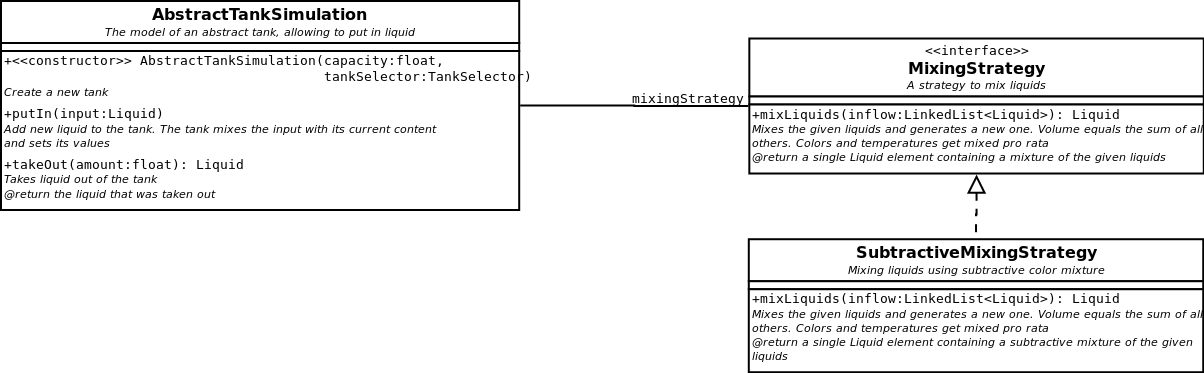
\includegraphics[scale=0.35]{design/pattern-screenshots/strategy-MixingStrategy.png}
  \caption{Ausschnitt aus dem Klassendiagramm: Strategie beim Mixen von Flüssigkeiten}
\end{figure}
In der Klasse \emph{AbstractTankSimulation} müssen Flüssigkeiten gemischt werden, wenn neue Flüssigkeiten in Tanks eingefügt werden.
Dafür müssen Temperaturen und Farben gemischt werden. Zur Farbmischung gibt es unterschiedliche Algorithmen, wie subtraktive oder additive
Farbmischung. Außerdem ist es denkbar, die Mischung der Temperaturen unterschiedlich zu implementieren (z.B. durch einen genauen und einen schnelleren,
approximativen Algorithmus).

Um diese Algorithmen, falls in Zukunft andere implementiert werden, einfach austauschbar zu machen, wurde
das Strategie-Muster angewandt. Dieses Muster hat das Ziel, eine Familie von Algorithmen zu definieren, zu kapseln und austauschbar zu machen.

Dabei ist \emph{MixingStrategy} das Interface, dass die Strategie definiert, und \emph{AbstractTankSimulation} die Kontextklasse, die die Algorithmen
benutzt. Momentan ist nur eine konkrete Strategie implementiert, und zwar die \emph{SubtractiveMixingStrategy}.

\pagebreak
\subsection{Beobachter-Muster: Observer bei Elementen des Models}
\begin{figure}[H]
  \centering
  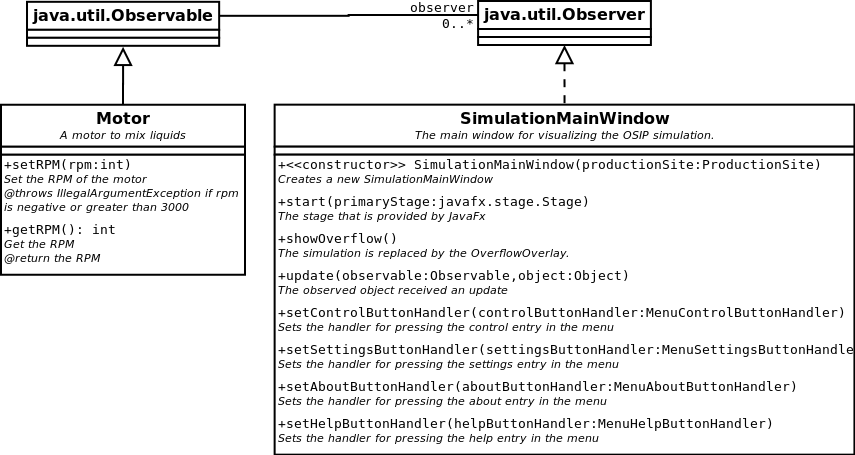
\includegraphics[scale=0.35]{design/pattern-screenshots/observer-Model.png}
  \caption{Ausschnitt aus dem Klassendiagramm: Observer bei Elementen des Models}
\end{figure}
Das derzeit geplante View-Modul holt sich periodisch den neuen Zustand des Models. Es wäre aber auch denkbar, ein View-Modul zu implementieren,
das sich nur aktualisiert, wenn sich Werte im Model geändert haben. Außerdem löst die Steuerung die Alarme der OPC UA Server immer dann aus, wenn die Alarme im Model
ausgelöst werden. Es ist also nötig, einen Mechanismus zu verwenden, mit dem das View-Modul und die Steuerung sich über Änderungen im Model informieren
lassen können.

Dazu haben wir das Beobachter (engl. Observer)-Muster verwendet. Dies definiert eine \emph{1 zu n}-Abhängigkeit zwischen dem Model und (z.B.) dem View.
Dabei wird jedoch eine möglichst lose Kopplung aufrecht erhalten. Darum ist das Beobachter-Muster sehr allgemein gehalten. Dabei kann ein OPC UA Server (konkreter Beobachter)
sich bei den relevanten Klassen (konkretes Subjekt) als Beobachter registrieren, und wird dann bei jeder Änderung informiert, in dem die Methode \emph{update()}
vom Subjekt aufgerufen wird. Dazu muss der konkrete Beobachter nur ein sehr kleines Interface (\emph{java.util.Observer}) implementieren.

Das Beobachter Muster wird verwendet, um die View oder die Steuerung über Änderungen in den Zuständen der Tanks, den Leitungen, dem Motor sowie über
das Auslösen von Alarmen zu informieren. Deswegen ist die Klasse \emph{AbstractTank}, \emph{Pipe}, \emph{Motor} und \emph{TankAlarm} als Subjekt implementiert
(d.h. sie erben von \emph{java.util.Observerable}). Damit können alle Teile der Anwendung sich über Veränderungen im Model informieren lassen.

\pagebreak
\subsection{Fassaden-Muster: Views der Überwachungskonsole}
\begin{figure}[H]
  \centering
  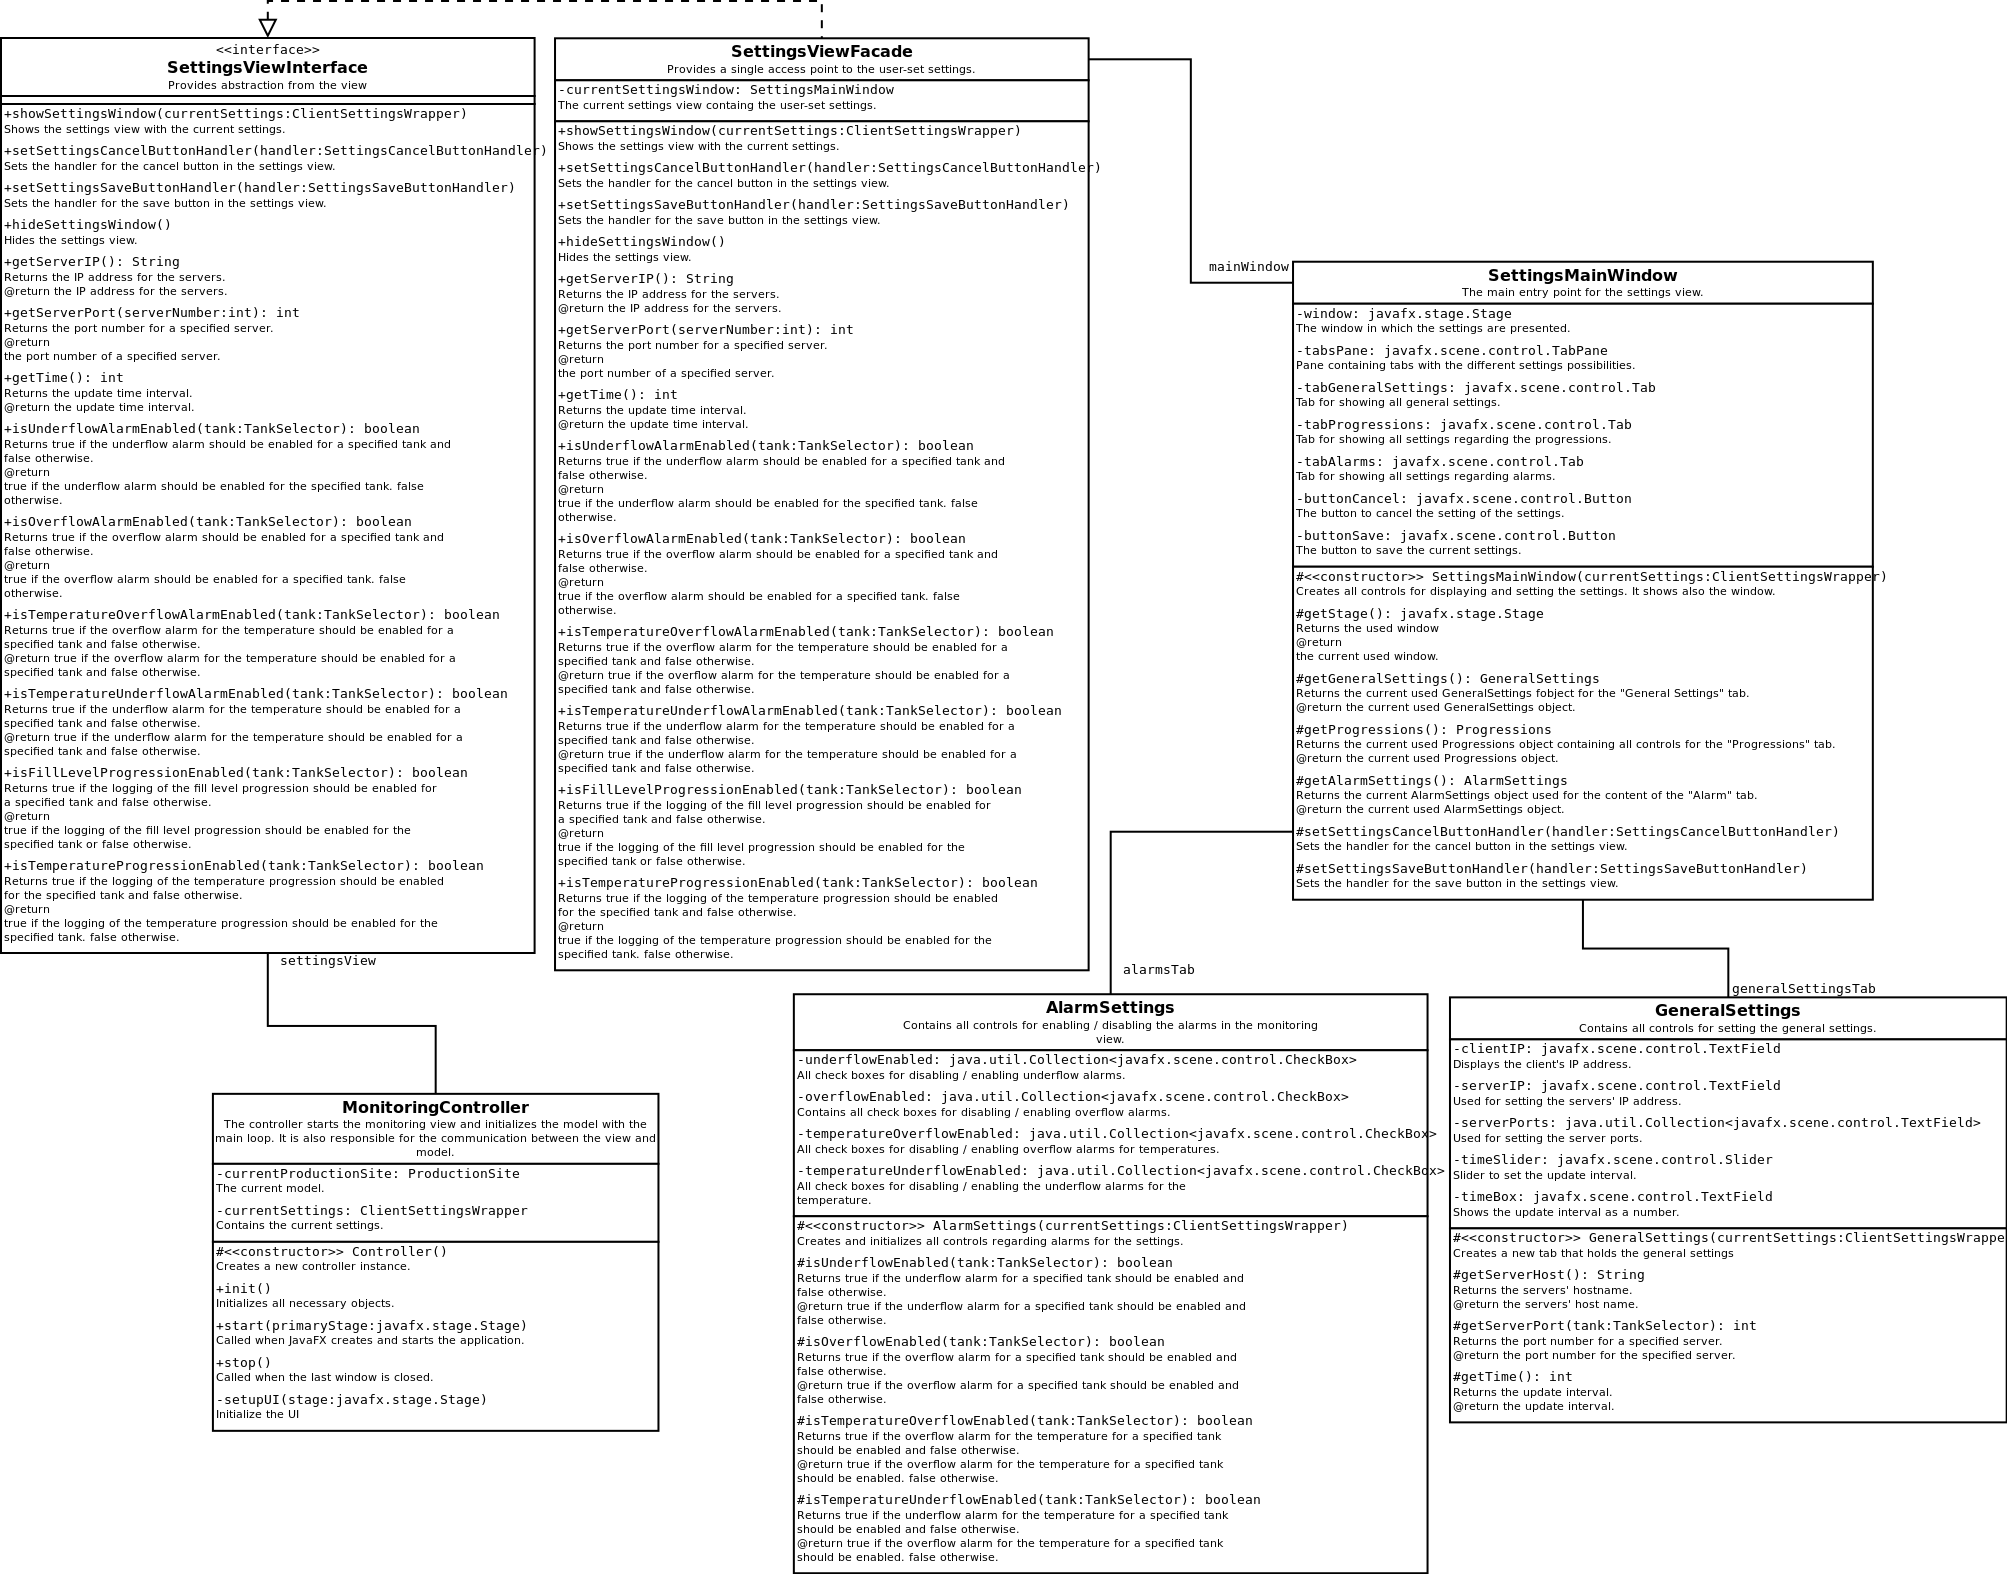
\includegraphics[scale=0.22]{design/pattern-screenshots/fascade-SettingsView.png}
  \caption{Ausschnitt aus dem Klassendiagramm: Fassade des Views der Überwachungskonsole}
\end{figure}
Jeder Zugriff auf das Haupt- oder Einstellungsfenster der Überwachungskonsole von außerhalb der Views erfolgt über jeweils eine eigene, konkrete Fassade:
\emph{MonitoringViewFacade} für das Hauptfenster und \emph{SettingsViewFacade} für das Einstellungsfenster. Beide Fassaden leiten sich von den eigentlichen Fassaden, die in Form
von Interfaces (\emph{MonitoringViewInterface} und \emph{SettingsViewInterface}) vorliegen, ab.

Die Fassaden an sich ermöglichen zunächst einen einheitlichen und zentralen Zugriff auf die notwendigsten Funktionen und Werte der Views, die außerhalb benötigt werden. Somit
bleiben die Entwurfs- und Implementierungsdetails der Views (Aufbau, verwendete GUI-Komponenten) zum größten Teil verborgen. Gleichzeitig können die Views nicht beliebig
modifiziert werden, womit gewährleistet wird, dass sie genau das anzeigen, was sie anzeigen sollen.

Vor allem die Interfaces sorgen für eine stärkere Trennung zwischen View und Controller, die die Views leichter austauschbar machen. Eine neue View muss nur Fassaden, die das
\emph{MonitoringViewInterface} bzw. \emph{SettingsViewInterface} implementieren, bereitstellen und kann alle Sensordaten und Alarme auf eine eigene Art und Weise darstellen.

\pagebreak
\subsection{Befehlsmuster: ButtonHandler im Controller der Überwachungskonsole}
\begin{figure}[H]
  \centering
  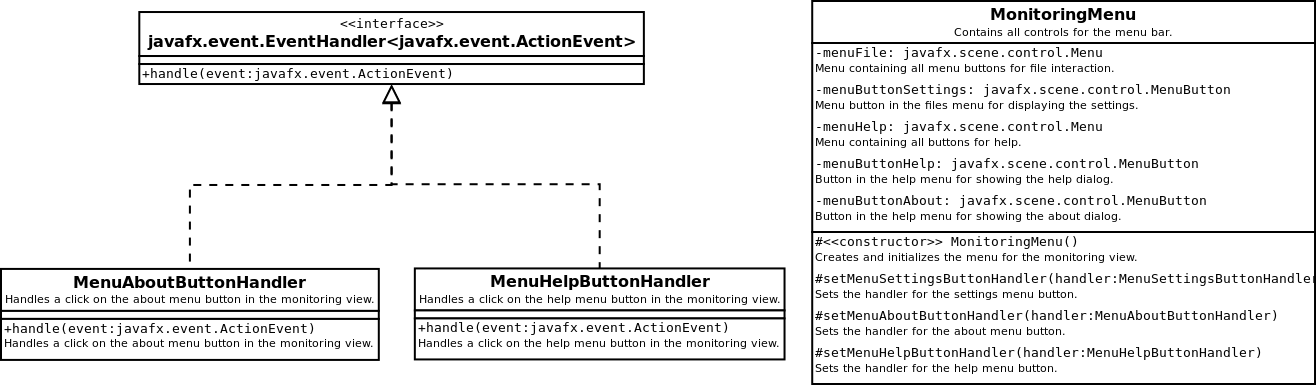
\includegraphics[scale=0.33]{design/pattern-screenshots/command-ButtonHandler.png}
  \caption{Ausschnitt aus dem Klassendiagramm: ButtonHandler der Überwachungskonsole}
\end{figure}
Haupt- und Einstellungsfenster der Überwachungskonsole beinhalten Knöpfe, mit denen der Benutzer verschiedene
Ereignisse auslösen kann. Zur Behandlung dieser Ereignisse wird das Befehlsmuster genutzt, das JavaFX bereits
unterstützt. So handelt es sich beim Interface \emph{javafx.event.EventHandler<? extends javafx.event.Event>}
um den abstrakten Befehl, der Bestandteil der Knöpfe von JavaFX (konkret hier: \emph{javafx.scene.control.Button} bzw. 
\emph{javafx.scene.control.\\MenuButton}) ist. Die konkreten Befehle stellen die \emph{ButtonHandler}-Klassen
im Controller dar, die das Interface implementieren und über ihre Konstruktoren die Empfänger der
Ereignisbehandlung erhalten.

Die Verwendung des Befehlsmusters ermöglicht es, ein bestimmtes Ereignis in einem dafür vorgesehenen Handler
zu bearbeiten und dieses damit in einem Objekt zu kapseln. Jeder Handler lässt sich eindeutig einer Aufgabe
und einem Ereignis zuordnen, sodass keine Verschränkung zwischen zwei verschiedenen Handlern auftritt.
Außerdem lässt sich leichter ein weiterer Handler hinzufügen oder ein bestehender Handler austauschen.

\pagebreak
\subsection{Singleton-Muster: Translator}
\begin{figure}[H]
  \centering
  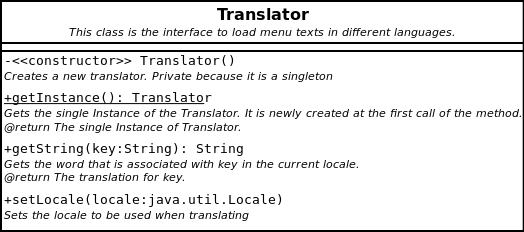
\includegraphics[scale=0.4]{design/pattern-screenshots/singleton-Translator.png}
  \caption{Ausschnitt aus dem Klassendiagramm: Translator als Singleton}
\end{figure}
Translator hat die Aufgabe, Menütexte in verschiedenen Sprachen zu laden.
Dabei lädt er zur gewählten Sprache eine Datei, in der Schlüssel zu Worten in der gewählten Sprache
zugeordnet werden. Jedes Mal, wenn ein Translator erzeugt wird, muss eine solche Datei
für eine Sprache geladen werden. Um dieses wiederholte Laden zu verhindern, ist Translator ein Singleton.
Es kann somit nur eine Translator-Instanz erzeugt werden und eine bereits geladene Datei
wird nicht erneut geladen. Falls die Sprache gewechselt wird, muss allerdings eine andere Datei geladen werden.

\pagebreak
\subsection{Schablonenmethode: Tanks in der GUI der Fertigungssimulation}
\begin{figure}[H]
  \centering
  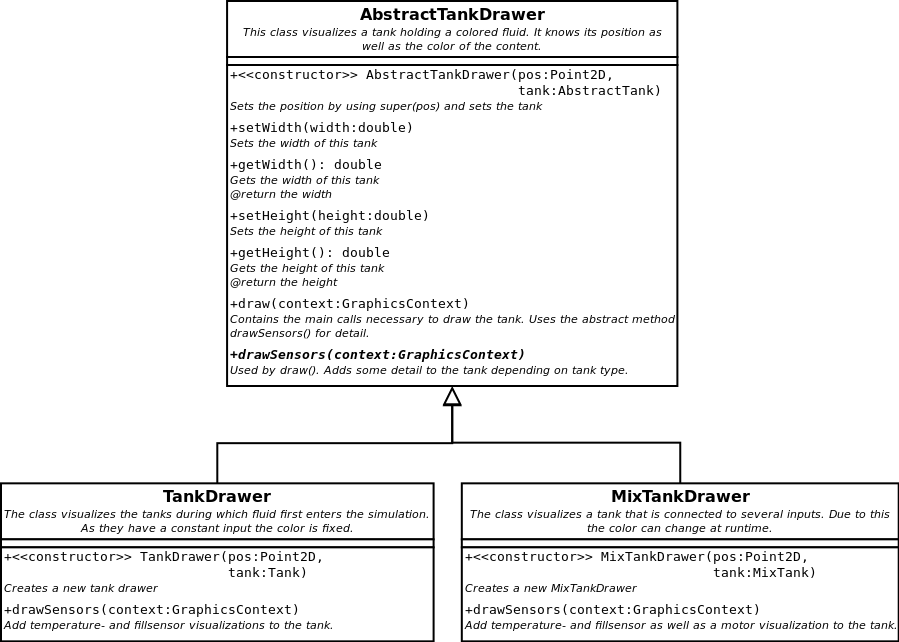
\includegraphics[scale=0.4]{design/pattern-screenshots/template-TankDrawer.png}
  \caption{Ausschnitt aus dem Klassendiagramm: Schablonenmethode im TankDrawer}
\end{figure}
Die Klassen \emph{TankDrawer} und \emph{MixTankDrawer} dienen der Visualisierung der Tanks in der Fertigungssimulation. Da sich die Tanks grunds\"atzlich
sehr \"ahnlich sind und sich in der Darstellung nur in der Menge der Sensoren unterscheiden, wurde die \emph{draw()}-Methode als Schablonenmethode umgesetzt.
Dazu wurde die Oberklasse \emph{AbstractTankDrawer} kreiert, die bereits Teile von \emph{draw()} implementiert und anschlie{\ss}end \emph{drawSensors()}
aufruft. Die Methode \emph{drawSensors()} ist in AbstractTankDrawer abstrakt und wird erst von den Unterklassen implementiert.\\
So werden die gemeinsamen Teile des Algorithmus zur Darstellung in eine gemeinsame Klasse ausgelagert, um Code-Duplikationen zu vermeiden. Auch \"Anderungen
werden so leichter umzusetzen, da der Code nur noch an einer statt an mehreren Stellen ge\"andert werden muss.

\pagebreak
\subsection{Value-Object: Liquid}
\begin{figure}[H]
  \centering
  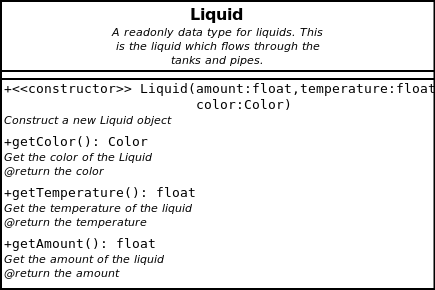
\includegraphics[scale=0.5]{design/pattern-screenshots/value-Liquid.png}
  \caption{Ausschnitt aus dem Klassendiagramm: Liquid als Value-Object}
\end{figure}
Die Klasse \emph{Liquid} dient der \"Ubermittlung von Werten aus einem Tank in einen anderen durch die \emph{Pipe}. Sie ist als Value-Object realisiert.
Das hei{\ss}t, sie erh\"alt bei der Erzeugung feste Werte, die sich sp\"ater nicht mehr \"andern k\"onnen. An Methoden werden nur Getter f\"ur die
verschiedenen Variablen angeboten. So wird sichergestellt, dass die \"ubermittelten Daten nicht ver\"andert werden.

\pagebreak
\phantomsection
\addcontentsline{toc}{section}{\listfigurename}
\listoffigures

\end{document}
